\documentclass[a4paper,english]{article}
\usepackage{graphicx}
\usepackage{listings}
%% Use utf-8 encoding for foreign characters
%%\usepackage[T1]{fontenc}
%%\usepackage[utf8]{inputenc}
%%\usepackage{babel}
%%
%%%% Vector based fonts instead of bitmaps
%%\usepackage{lmodern}
%%
%%%% Useful
%%%\usepackage{fullpage} % Smaller margins
%%\usepackage{enumerate}
%%
%%%% Theorem
%%\usepackage{amsthm}
%%
%%%% More math
%%\usepackage{amsmath}
%%\usepackage{amssymb}

%% Document Header
\title{Section3}
\author{Elliott Ashby}
\date{\today}

\begin{document}
    \maketitle
    \section{q1}
    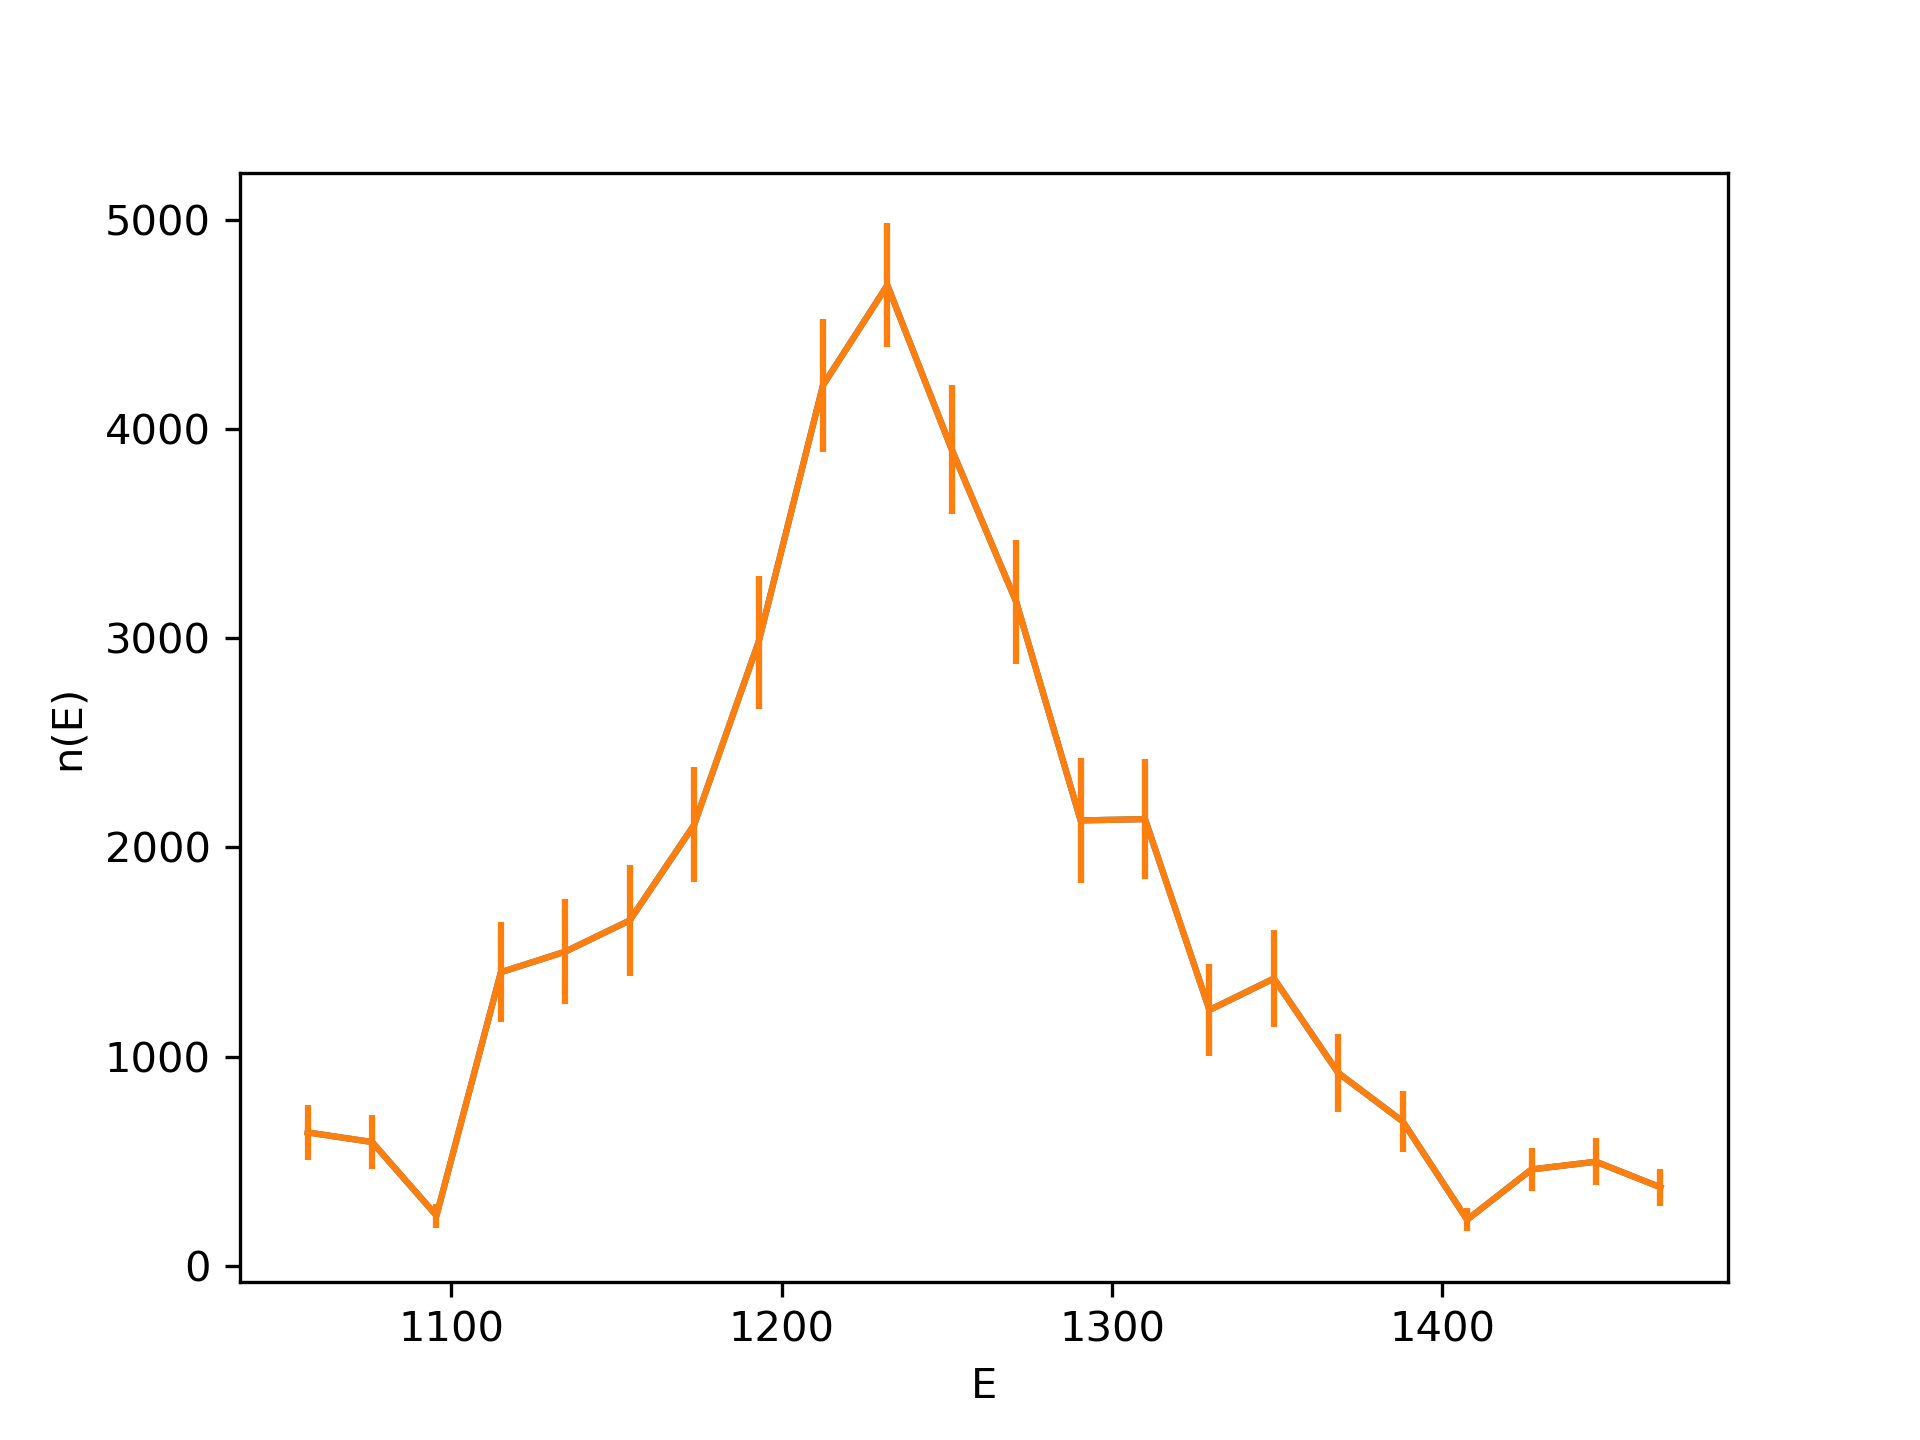
\includegraphics[scale=0.8]{./q3_1.png}
    \section{q2}
        As E increases from 1000 n(E) increases at an increasing rate
        until around 1200 where the gradient change decreases to a peak at 
        around 1250. This shape is mirrored on the other side ending around
        1500.
    \section{q3}
    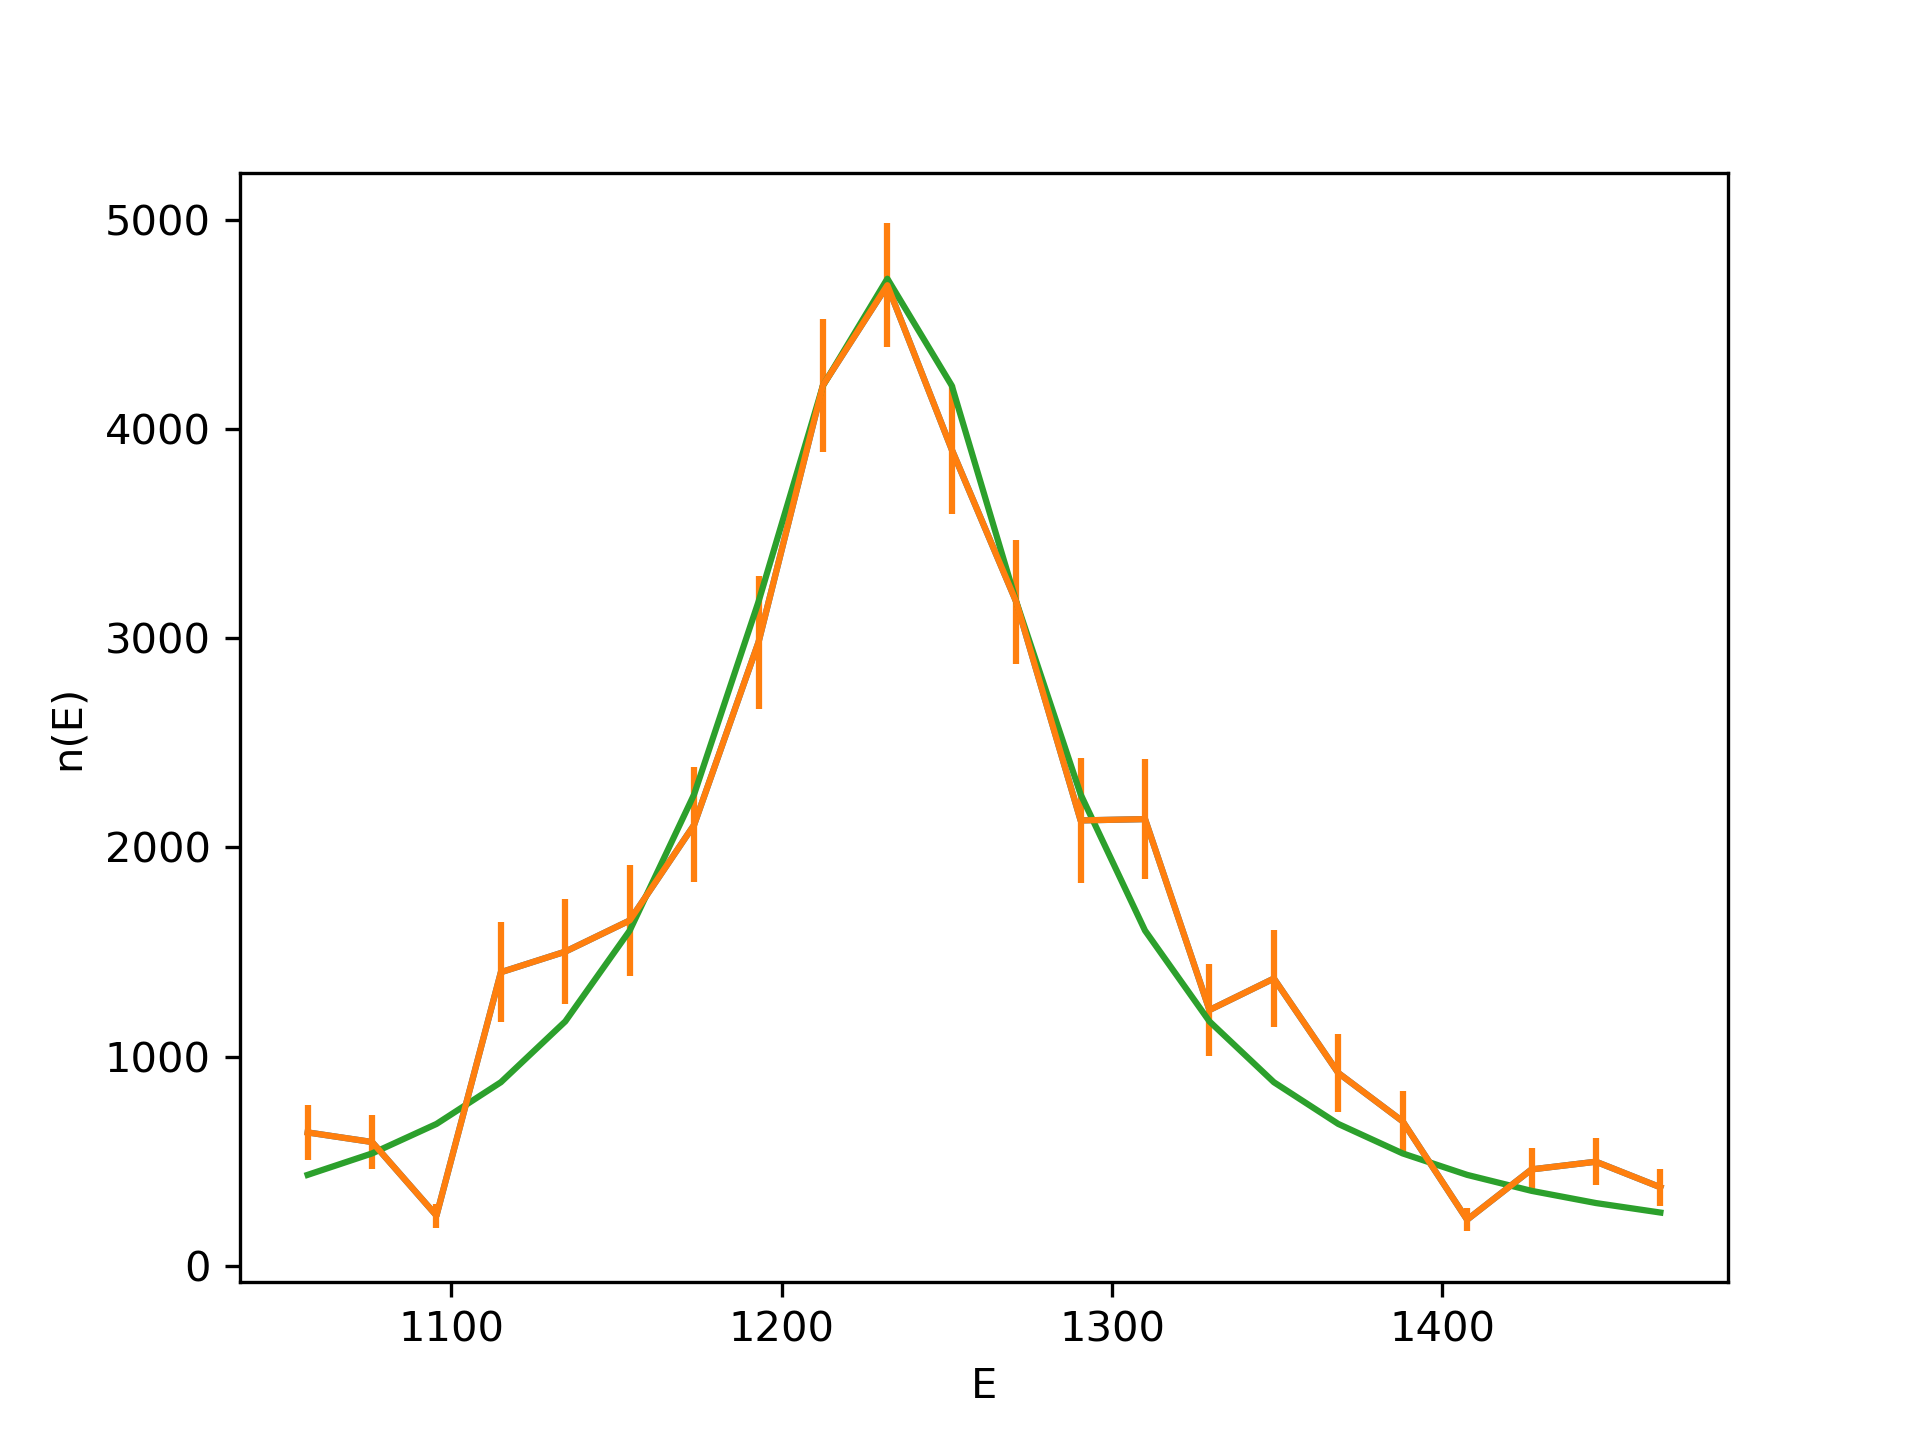
\includegraphics[scale=0.8]{./q3_1th.png}
        \begin{equation}
            w = \frac{600\sqrt{163}}{\sqrt{4687}}
        \end{equation}
        Changing $w$ effects the maximum value of the peak of the theoretical curve
        without changing the minimum values at roughly $n(E) = 500$. Increasing $w$
        decreases the maximum (since $w^2$ is divided by in $n(E)$). Whereas decreasing
        $w$ increases the maximum of $n(E)$.
    \section{q4}
        \lstinputlisting[language=Python]{./q3_4.py}
        This function takes in the values of the residuals and their errors and 
        returns a sum over each residual divided by their error squared.
    \section{q5}
        Manually using trial and error to reduce the discrepancy results in a minimum discrepancy of 86.76
        which is when $w = 113.15$. The method used is just iterating on the 
        value of $w$ and returning the value of the discrepancy each time.
    \section{q6}
        Using the gmin function like:
        \lstinputlisting[language=Python]{./q3_6.py}
        This returns the only minimum in the curve since in the negatives, f(x) is 
        decreasing to a asymptote.
        \\ This returns: \\ $\rightarrow$ (0.7034674247387416, 3.4422772944949744) \\ 
        which is the (x, y) coords of the minimum.
    \section{q7}
        Using gmin() on the discrepancy function reveals a minimum $w$ of 
        113.14847521305097 where the discrepancy is 86.76529920076851.
        using these values in a plot yields:
        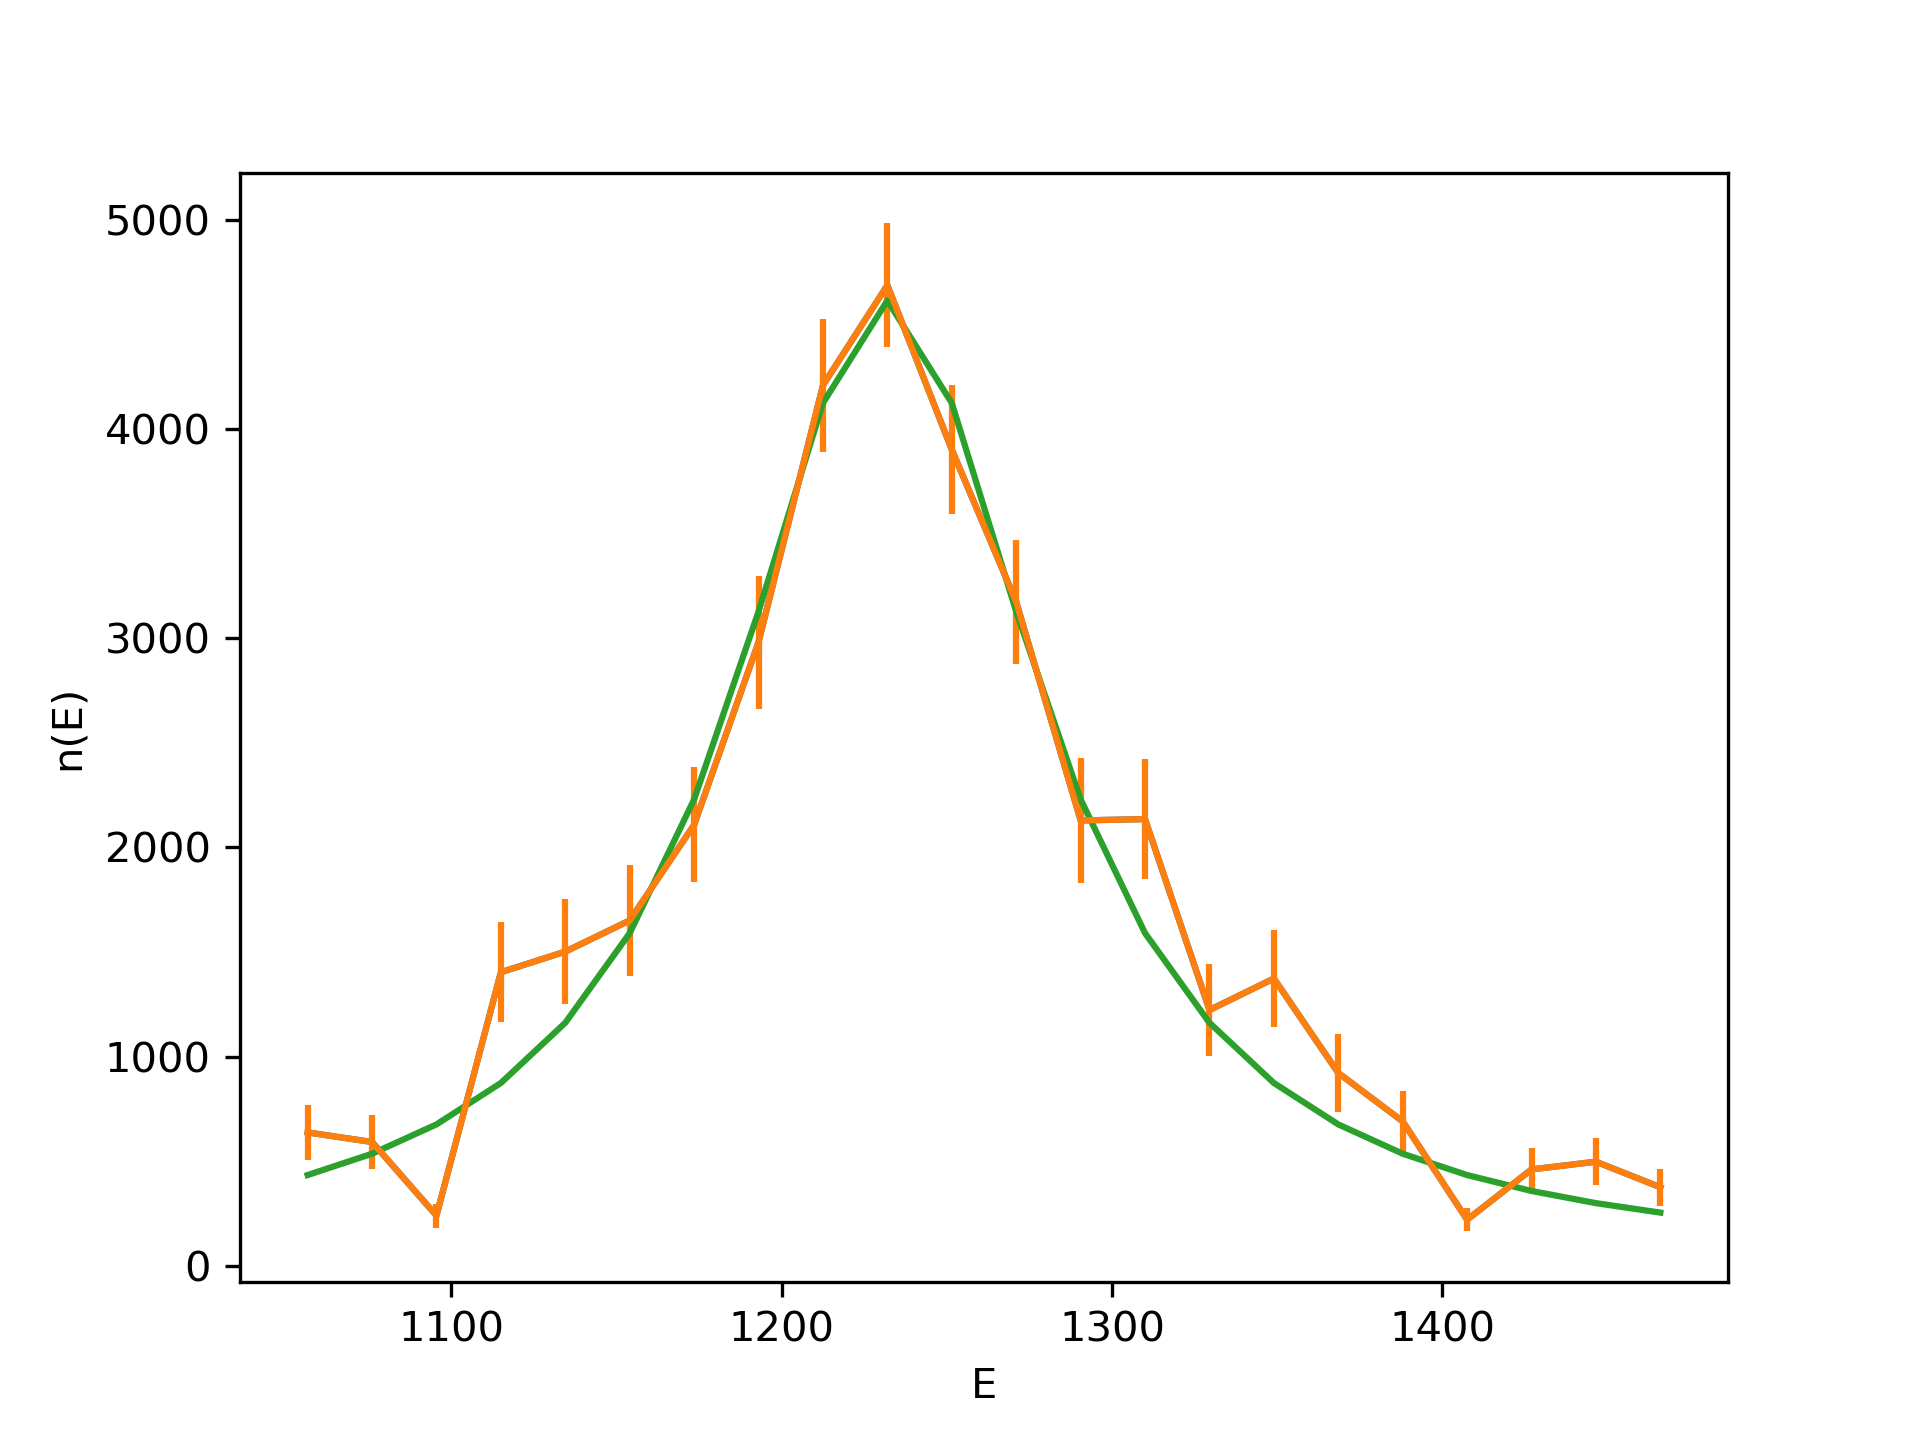
\includegraphics[scale=0.8]{./q3_7.png}
    \section{q8}
        \lstinputlisting[language=Python, firstline=6, lastline=14]{./q3_8.py}
        This outputs a value of $w$ of 113.14847521 with an uncertainty of 4.84317108
        
\end{document}
